% -*- root: ../main.tex -*-
%!TEX root = ../main.tex
% this file is called up by main.tex
% content in this file will be fed into the main document
% vim:textwidth=80 fo=cqt

\subsection{The transfer operator and its model form}
In a classical system identification  task, the discrete-time transfer functions
for the systems  under consideration need to be  determined. These discrete-time
transfer functions are  based on Z-transforms in the  frequency domain. However,
for the purpose of working in time-domain, an analogous linear operator $q$ that
performs a  forward shift on  its input \ie{} $  {q u[k] \longmapsto  u[k+1]} $.
Similarly, applying the  backward shift operator $ q^{-1} $  on the input yields
its value at the previous time-step \ie{} $ {q^{-1} u[k] \longmapsto u[k-1]}$.

\begin{figure}[!htb]
    \centering
    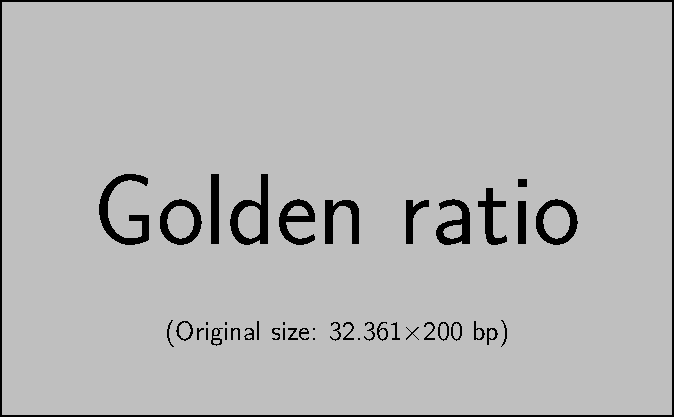
\includegraphics{placeholder_images/example-image-golden.pdf}
    \caption[Block diagram representing a generic discrete-time \glsfmtshort{lti} system]{%
        Block  diagram representing  a  generic discrete-time  \glsfmtshort{lti}
        system. The  control input $u[k]$ is  acted upon by the  system dynamics
        $G[k]$  whereas a  white  noise  input $e[k]$  is  shaped  by the  noise
        dynamics $H[k]$. The  overall output $y[k]$ consists  of a superposition
        of the contribution from both these components.
    }%
    \label{fig:genericltisyswithnoise}
\end{figure}

\Cref{fig:genericltisyswithnoise} shows  a generic \gls{lti} system  wherein the
measurements are corrupted by noise. The  system dynamics are represented by the
transfer operator $G(q)$\footnote{The term transfer  operator in the time domain
mathematically  corresponds  to the  term  transfer  function in  the  frequency
domain.  Mathematically,  $G(q) =  G(z)\bigr\rvert_{\mathrlap{z=q}}$.}  that  acts on  the
applied  input  $u[k]$,  whereas  the  noise dynamics  are  represented  by  the
disturbance operator  $H(q)$ that  acts to  filter (or  shape) an  assumed white
noise input $e[k]$.

Assuming linearity and time-invariance throughout, the overall output can be
written as the linear combination
\begin{equation}\label{eq:outputwithsysandnoise}
    % \SwapAboveDisplaySkip
    y[k] = G(q)u[k] + H(q)e[k]
\end{equation}
where $G(q) = \frac{B(q)}{A(q)}$ and $H(q) = \frac{C(q)}{D(q)}$ are the transfer
operators describing the dynamics of the system and disturbance respectively.

$A(q), B(q), C(q)$ and $D(q)$ are rational polynomials in $q$. The two transfer
operators $G(q)$ and $H(q)$ can be represented by
\begin{align}
    G(q) &= q^{-n_k}\frac{b_1q^{-1} + \dots  + b_{n_b}q^{-{n_b}}}{1 + a_1q^{-1} + \dots  + a_{n_a}q^{-{n_a}}} \\
    H(q) &= q^{-n_l}\frac{c_1q^{-1} + \dots  + c_{n_c}q^{-{n_c}}}{1 + d_1q^{-1} + \dots  + d_{n_d}q^{-{n_d}}}
\end{align}
where $(n_k,n_l)$ represent  the number of transport  delay samples, $(n_b,n_c)$
the number  of feedforward coefficients  and $(n_a,n_d)$ the number  of feedback
coefficients in $G(q)$ and $H(q)$ respectively.


In  this  system  identification  task  at hand,  the  output  measurements  are
collected from a  \emph{noise-free} simulation of the \gls{p2d}  model \ie{} the
disturbance transfer operator in~\cref{eq:outputwithsysandnoise} is zero
\begin{align}
    y[k] &= G(q)u[k] + \cancelto{0}{H(q)}e[k]
\shortintertext{Hence, the time-domain output  reduces  to}
y[k] &= G(q)u[k] \label{eq:outputwithsysonly}
\end{align}

Thus, the system identification task becomes one that of estimating
\begin{enumerate}
    \item The number of transport delay samples $n_k$.
    \item The number of feedforward coefficients (zeros) $n_b$.
    \item The zeros themselves $b_1, b_2, \dots b_{n_b}$.
    \item The number of feedback coefficients (poles) $n_a$.
    \item The pole locations $a_1, a_2 \dots a_{n_a}$.
\end{enumerate}
for  each  of  the  two  transfer operators  $G_1(q)$  and  $G_2(q)$  \ie{}  the
electrolyte  time-evolution subsystems  in the  negative and  positive electrode
region respectively.

\subsection{Estimation of transport delay}

The transport delay $n_k$ can be estimated visually by inspecting the step
response of the systems under consideration.

In~\cref{fig:linearity},   step  inputs   of   $I_1   =  \SI{60}{\ampere},   I_2
=    \SI{12}{\ampere},$   and    $I_3   =    \SI{36}{\ampere}$   were    applied
to    the   two    subsystems.    Inspecting   closely    all   the    responses
\ie{}   $\widetilde{Q}_{\text{e,n}_1},    \widetilde{Q}_{\text{e,n}_2}   $   and
$\widetilde{Q}_{\text{e,n}_3}$    in    the     negative    electrode    region,
and    $\widetilde{Q}_{\text{e,p}_1},    \widetilde{Q}_{\text{e,p}_2}   $    and
$\widetilde{Q}_{\text{e,p}_3}$  in the  positive electrode  region, it  is clear
that all these outputs start exactly at  zero. Therefore, there is no delay term
to be considered for the transfer operators \ie{} $n_k = 0$ for both subsystems.

\subsection{Choice of model structure}\label{subsec:modelstrucchoice}

Among      the      transfer-function       model      structures      mentioned
in~\cref{subsec:parametric}, the \gls{arx} model  structure is too simplistic to
consider. Despite  the fact that  its numerical computation involves  only basic
linear algebra operations,  that can be efficiently handled  on modern computing
systems, it  is considered to produce  poor estimates of the  system's poles and
zeros. In the absence of contributions from the noise-term, the all-encompassing
model structure used by the Box-Jenkins approach is deemed to be unnecessary for
the  problem  at hand.  Therefore,  the  two  model structures  considered  were
\gls{armax} and \gls{oe} for the coefficient determination.

\subsection{Starting guesses for coefficient orders}\label{subsec:initguesscoefforder}

At first, the training profile of~\cref{fig:sysidtrainingcurrent} is
debiased (through mean removal) and applied as the input current profile in a \gls{p2d}
simulation. The outputs of this simulation are suitably post-processed as per
the following sequence of steps.
\begin{enumerate}
    \item The concentrations solved at various node locations within each
        electrode are numerically integrated over the corresponding electrode
        thicknesses using trapezoidal rule.
    \item The resulting integral value is multiplied with the porosity of the
        corresponding electrode region to obtain $Q_{\text{e,n}_\text{train}}(t)$ and
        $Q_{\text{e,p}_\text{train}}(t)$.
    \item These quantities are then de-biased by subtracting their initial
        values to obtain $\widetilde{Q}_{\text{e,n}_\text{train}}(t)$ and
        $\widetilde{Q}_{\text{e,p}_\text{train}}(t)$.
\end{enumerate}

The        same        procedure        is        repeated        for        the
validation       current      profile       of~\cref{fig:sysidvalidationcurrent}
to         obtain         $\widetilde{Q}_{\text{e,n}_\text{val}}(t)$         and
$\widetilde{Q}_{\text{e,n}_\text{val}}(t)$.  These data  sets are  used for  all
subsequent sub-tasks involved in this system identification exercise.

In  order to  reduce  the search  window for  the  coefficient determination  in
the  parametric transfer  function methods,  the hand-estimation  of coefficient
order  through non-parametric  methods may  be performed.  This coarse  estimate
can  act as  a  feeder to  help  in  the faster  convergence  of the  non-linear
optimisation algorithms  used in the parametric  methods. In this case,  a basic
spectral analysis  using a Hanning  window implemented using the  MATLAB command
\texttt{spa.m} is applied to the time-domain data to transform it into frequency
response data.

\begin{figure}[!htb]
    \centering
    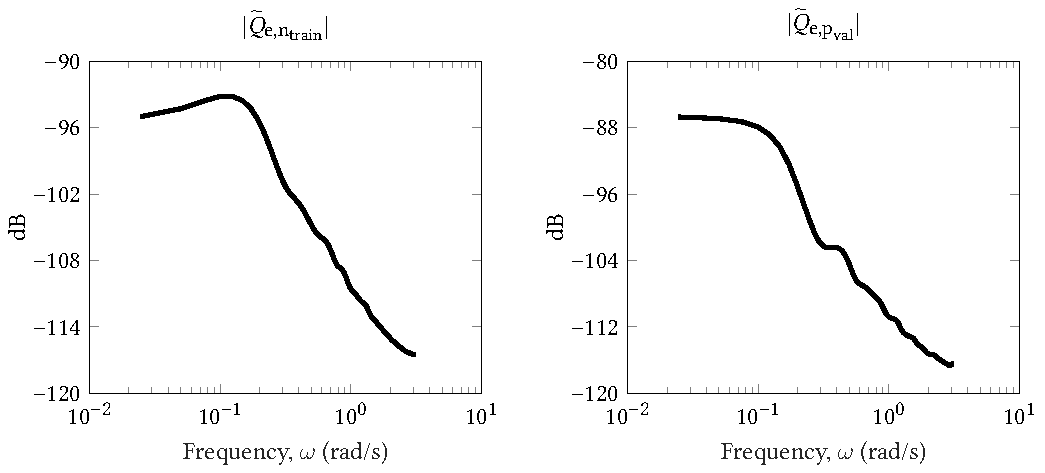
\includegraphics[width=\textwidth]{bode_mag.pdf}
    \caption[Bode magnitude plots of the electrolyte time-evolution sub-systems]{%
        Bode magnitude  plots showing the  estimated frequency response  for the
        two  subsystems under  consideration.  The frequency  response data  was
        obtained  through a spectral  analysis \ie{}  by computing  the ratios  of
        spectra of the de-biased input  and output sequences. The sequences were
        smoothed using a Hanning window before computing the ratio.
    }%
    \label{fig:initialbodemag}
\end{figure}

\Cref{fig:initialbodemag}  shows  the  Bode  magnitude  plot  of  the  frequency
response for
\begin{enumerate*}[label=\emph{\alph*})]
    \item the training set in the negative electrode region, and
    \item the validation set in the positive electrode region.
\end{enumerate*}
In the  plots, a broad  combination of  the two data  sets in the  two electrode
region  is  depicted  to  achieve  a  compact  representation  of  all  possible
permutations and to avoid redundancies by plotting visually similar information.
It is important to note that these Bode diagrams obtained by such non-parametric
methods only represent  a crude approximation of the  physical dynamics intended
to help in initial estimates of the system behaviour.

Some preliminary understanding of the  various characteristics of the system can
be gleaned from these Bode diagrams.  The first visually striking feature is the
similarity  in the  approximate frequency  characteristics in  the negative  and
positive electrode  regions, even when  excited by completely different  data in
the time domain. This confirms the author's assumptions of equal `complexity' in
the symbolic  regression search discussed in~\cref{subsec:symbolicreg}.  This is
also  congruent with  the physical  behaviour of  the electrolyte  in these  two
regions.

\subsubsection*{Finite DC gain}
By visual  extension of  the frequency responses  towards lower  frequencies, it
is  clear  that  the  DC  gains  of  both  the  systems  are  finite  and  below
unity.  This  behaviour  can  clearly  be  seen  in  the  time-domain  responses
of~\cref{fig:linearity}.  For  the plotted  time-horizon,  this  effect is  most
visible for the case of the \SI{12}{\ampere} constant current input, wherein the
responses of both regions settle to a finite value after an initial transient.

There is \approx\SI{10}{\decibel} variability in  the low frequency gain between
the two Bode  plots in~\cref{fig:initialbodemag}. This can be  attributed to the
following  factors. A  compromise with  the spectral  estimation method  is that
using a higher number of frequency bins  results in lower resolution per bin and
vice-versa. By  varying the number  of frequency bins  and focussing on  the low
frequency range, the resolution of the DC  gain can be improved. The rest of the
variability can  be attributed to the  fact that the training  and test profiles
behave differently and do not excite the same dynamics. In particular, the swept
frequency cosine (chirp) signal in the training set was specifically designed to
draw out  the low frequency  dynamics with a  high fidelity. Finally,  the small
range of variation in the DC gain could also be due to the intrinsic small-scale
variations of  the electrolyte  behaviour in  these two  regions. Although  on a
macroscopic frequency scale the two regions behave similarly, the differences in
electrode thicknesses and porosities could contribute to the small difference in
the  DC gain.  This  helps  to confirm  that  two \emph{non-identical}  transfer
functions are being sought for --- one for each electrode region.

Finally, the finiteness  of the DC gain  helps to narrow down  the search window
for the parametric model structures. In particular, this fact indicates that the
model structures to be trialled must not  have any integrator terms (or poles at
the origin of the complex plane).

\subsubsection*{Resonance and model order}

First  order  transfer   functions  do  not  exhibit   characteristic  peaks  or
resonances  in  their  frequency  responses.  However,  for  the  Bode  plot  on
the   left   of~\cref{fig:initialbodemag},   a   pronounced   resonance   around
\SI{0.15}{\radian\per\second} is observable. This has  an enormous impact --- it
presents  an important  clue  that the  first  order time-evolution  \glspl{ode}
of~\cref{eq:negliionmolesquadratic}   and~\cref{eq:posliionmolesquadratic}   are
inadequate to represent the system dynamics.

An apparent  contradiction to  the first-order inadequacy  claim stems  from the
Bode plot  on the  right hand side  in~\cref{fig:initialbodemag}. In  this case,
there are no resonances in the  magnitude response indicating that a first order
model description is sufficient. However, a vital aspect to be noted here is the
nature of the  validation current profile when compared to  that of the training
current profile.  The coarse  frequency response data  obtained by  the spectral
method is sensitive to the actual  input sequence employed. From systems theory,
the  resonances at  a frequency  occur  due to  the presence  of lightly  damped
complex conjugate poles at that frequency. The periodic \gls{rgs} was explicitly
designed in the  training set and is  however absent in the  validation set. The
unique characteristics  of the validation  set and its influence  on coefficient
order is discussed next.

As per  the arguments presented  in the  preceding discussions, there  exists an
implicit constraint that  the behaviour of the time-evolution  subsystems in the
two electrode  regions are  expected to be  of similar  `complexity'. Therefore,
based  on the  presence of  the resonance  in the  Bode magnitude  plot for  the
response to  training profile  in the  negative electrode region,  it has  to be
concluded that the two subsystems are \emph{at-least} of second order.

\subsubsection*{Estimation of number of poles and zeros}

The  high-frequency  roll-off  in  the   slopes  of  the  Bode  magnitude  plots
in~\cref{fig:initialbodemag} provide clues on the number of poles in the system.
The  corner  frequency $\omega_\text{c}$  in  both  cases  appear to  be  around
\SI{0.15}{\radian\per\second}.  The  high-frequency  slope of  both  systems  is
\approx\SI{20}{\decibel} per decade,  which implies that they  have at-least one
more pole than the number of zeros \ie{} $n_a \ge n_b + 1$.

In the  aspect of estimating the  number and locations of  zeros, the validation
profile outshines  the training profile. While  the Bode plot obtained  with the
training profile  does not indicate  the presence of  zeros in the  systems, the
plateau in \SIrange{0.3}{0.4}{\hertz} range for  the Bode plot of the validation
profile clearly contradicts this. Once again, hypothesising that the two systems
(in the two electrode regions)  have fundamentally identical behaviour with only
small differences owing  to differences in their parameter  values, there exists
at-least one zero in these systems around this frequency range.

Based on this  preliminary analysis, the estimates  are $n_k = 0$,  $n_a \ge 2$,
$n_b  \ge  1$. Only  asymptotic  approximations  to  corner frequencies  can  be
estimated from the Bode plots. Furthermore, the estimated locations are not used
in  the  parametric  system  identification  algorithms  and  is  of  much  less
importance than the model order estimates. With this initial understanding, the
parametric system identification procedure is carried out.

\subsection{Refinement of coefficient orders using deterministic criteria}

The initial estimate  of coefficient orders in~\cref{subsec:initguesscoefforder}
was performed  based only on  a visual inspection  of the Bode  magnitude plots.
Owing to  the fact that  the frequency  response data is  the result of  a crude
ratio of  spectra, there is a  high probability of missing  vital information on
the number and locations of poles and zeros. Hence only a lower bound on the
coefficient orders are available until this point. Next, a set of deterministic
criteria is used to widen and refine the coefficient order range.


Although   the   \gls{arx}   structure   is  deemed   to   be   too   simplistic
(see~\cref{subsec:modelstrucchoice}), owing to the fact that only linear algebra
operations are involved, as opposed  to numerical optimisation routines employed
in the  \gls{oe}, \gls{armax} and Box-Jenkins  structures, certain deterministic
criteria for  coefficient order  selection can  be incorporated  for coefficient
order selection.
This  can serve  as  a  refinement  of  the
initial number of  coefficients guessed from the Bode  magnitude plots discussed
in.

For any model structure used, its error can be defined as
\begin{align}
    % \SwapAboveDisplaySkip
    \varepsilon[k]      & = y[k] - \hat{y}_\text{m}[k] \label{eq:sysiderroronlyk}\\
    \shortintertext{where $y[k]$ are true measurements and}
    \hat{y}_\text{m}[k] & = G(q)u[k] \tag{\cref{eq:outputwithsysonly} revisited}
\end{align}
are the model outputs obtained by the assumed transfer operator $G(q)$ (which is
to be determined).

The  number of  numerator  and denominator  coefficients in  $G(q)$  as well  as
their  values are  to  be determined.  This  set of  unknowns  can be  collected
into a  parameter vector  $\theta$. Thus, as  per~\cref{eq:sysiderroronlyk}, the
error  sequence is  parametrised by  $\theta$, and  its notation  is amended  to
$\varepsilon[k;\theta]$.

For  an  input-output  data  set  consisting of  $N$  samples,  a  generic  cost
function that may  be applied for all the four  model structures \viz{\gls{arx},
\gls{armax}, \gls{oe} and Box-Jenkins} is
\begin{align}
    V_N(\theta) &= \sum_{k=1}^N L\left(\varepsilon\left[k;\theta\right]\right)
\shortintertext{where $L(\cdot)$ is a postive-valued scalar loss function.}
\intertext{For the \gls{arx} structure, the sum of squares of the error sequence
    may be used as the loss function yielding}
    V_N(\theta) &= \sum_{k=1}^N \varepsilon^2[k;\theta]
    \shortintertext{whose least squares solution $\hat{\theta}$ is desired}
    \hat{\theta} &= \text{arg}\,\underset{\theta}{\text{min}} V_N(\theta)
\end{align}

With this least squares problem applied to the \gls{arx} model structure, two
deterministic model order criteria have been defined ---
\begin{enumerate*}[label=\emph{\alph*})]
    \item \gls{aic}, and
    \item \gls{mdl}~\cite{Ljung1999}.
\end{enumerate*}


